\begin{figure}[!h]
    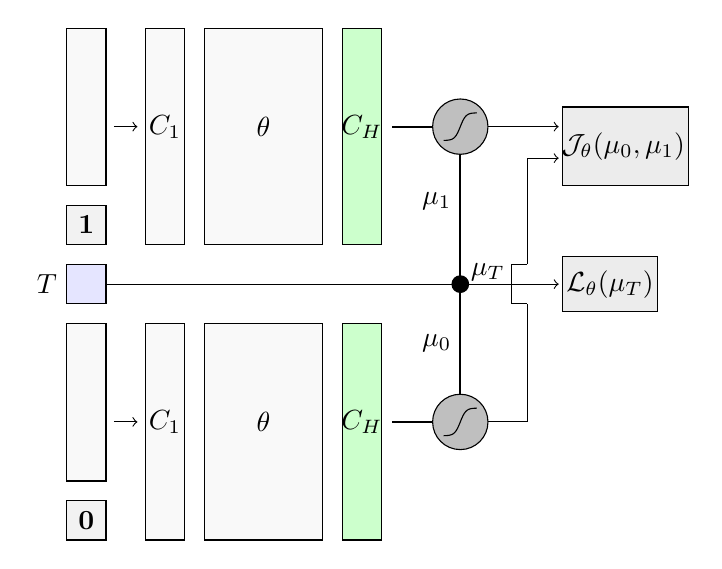
\begin{tikzpicture}
    
    \tikzset{dist/.style={path picture= {
    \begin{scope}[x=1pt,y=10pt]
      \draw plot[domain=-6:6] (\x,{1/(1 + exp(-\x))-0.5});
    \end{scope}
    }}}
    \tikzstyle{sigmoid}=[draw,fill=gray!50,circle,minimum size=20pt,inner sep=0pt,dist]
    
    \filldraw[fill=gray!5!white, draw=black]  (0,0) rectangle (0.5,2);
    \node at (-0.25,1) {$\X$};
    \filldraw[fill=gray!10!white, draw=black] (0,-0.75) rectangle (0.5,-0.25); 
    \node at (0.25,-0.5) {$\mathbf{1}$};

    \filldraw[fill=blue!10!white, draw=black] (0,-1.5) rectangle (0.5,-1); 
    \node(treatment) at (-0.25,-1.25) {$T$};
    
    \filldraw[fill=gray!5!white, draw=black] (0,-3.75) rectangle (0.5,-1.75);
    \node at (-0.25,-2.75) {$\X$};
    \filldraw[fill=gray!10!white, draw=black] (0,-4.5) rectangle (0.5,-4); 
    \node at (0.25,-4.25) {$\mathbf{0}$};

    \filldraw[fill=gray!5!white, draw=black] (1,-0.75) rectangle (1.5,2);
    \node at (1.25,0.75) {$C_1$};
    \draw [->] (0.6,0.75) -- (0.9,0.75);
    
    \filldraw[fill=gray!5!white, draw=black] (1,-4.5) rectangle (1.5,-1.75);
    \node at (1.25,-3) {$C_1$};
    \draw [->] (0.6,-3) -- (0.9,-3);
    
    
    \filldraw[fill=gray!5!white, draw=black] (1.75,-4.5) rectangle (3.25,-1.75);
    \node at (2.5,-3) {$\boldsymbol{\theta}$};
    
    \filldraw[fill=gray!5!white, draw=black] (1.75,-0.75) rectangle (3.25,2);
    \node at (2.5,0.75) {$\boldsymbol{\theta}$};

    \filldraw[fill=green!20!white, draw=black] (3.5,-0.75) rectangle(4,2);
    \node(lp1) at (3.75,0.75) {$C_H$};
    
    \filldraw[fill=green!20!white, draw=black] (3.5,-4.5) rectangle (4,-1.75);
    \node(lp0) at (3.75,-3) {$C_H$};
    
    \node (p1)[sigmoid] at (5, 0.75) {};
    \node (p0)[sigmoid] at (5, -3) {};
    
    \filldraw (5,-1.25) circle (3pt);
    \draw [->] (0.5,-1.25) -- (5,-1.25);
    
    \draw[thick] (lp1) -- (p1) node [midway,above=-0.06cm] {};
    \draw[thick] (p1) -- (p0) node [midway,above=-0.06cm] {};
    \draw[thick] (lp0) -- (p0) node [midway,above=-0.06cm] {};
    
    \node(mu) at (4.7,-0.2) {$\mu_1$};
    \node(mu) at (4.7,-2) {$\mu_0$};
    \draw [->] (5,-1.25) -- (6.25,-1.25);
    \draw  (5.35,-3) -- (5.85,-3);
    \draw  (5.85,-3) -- (5.85,-1.5);
    \draw  (5.85,-1.5) -- (5.65,-1.5);
    \draw  (5.65,-1.5) -- (5.65,-1);
    \draw  (5.65,-1) -- (5.85,-1);
    \draw  (5.85,-1) -- (5.85,0.35);
    \draw [->] (5.85,0.35) -- (6.25,0.35);
    \draw [->] (5.35,0.75) -- (6.25,0.75);
    
    \node(mut) at (5.35,-1.1) {$\mu_T$};
    
    \filldraw[fill=gray!15!white, draw=black] (6.3,-1.6) rectangle (7.5,-0.9);
    \node at (6.9,-1.25) {$\mathcal{L}_{\boldsymbol{\theta}}(\mu_T)$};
    
    \filldraw[fill=gray!15!white, draw=black] (6.3,0) rectangle (7.9,1);
    \node at (7.07,0.5) {$\mathcal{J}_{\boldsymbol{\theta}}(\mu_0,\mu_1)$};
    
    \end{tikzpicture}
    \caption{SMITE: Neural network architecture for uplift estimation.}
    \label{fig:nite}
\end{figure}
